\documentclass[12px]{article}
\usepackage[cjk]{kotex}
\usepackage[top=2cm, bottom=2cm, left=2.5cm, right=2.5cm]{geometry}
\usepackage{amsmath, amssymb}
\usepackage{enumerate}
\usepackage{graphicx}

\everymath{\displaystyle}

\title{응용통계학 8장 연습문제 풀이}
\author{20181653 이강희}
\date{}

\begin{document}
\maketitle

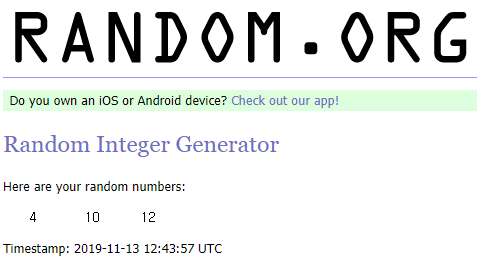
\includegraphics[scale=0.7]{random}

\section*{4번}
    n이 100으로 충분히 크므로, 중심극한정리에 의해 $\overline{X} \sim N(140, 0.04)$ 이다.
\begin{enumerate}[(1)]
    \item
    $\!\begin{aligned}[t]
        P(\overline{X} \geq 140.5) &= P(\frac{\overline{X}-140}{0.2} \geq 2.5) &\\
        &= P(Z \ge 2.5) = 1 - P(Z \leq 2.5) = 1 - 0.9938 = 0.0062
    \end{aligned}$

    \item
    $\!\begin{aligned}[t]
        0.95 &= P(-1.96 \leq Z \leq 1.96) &\\
        &= P(-1.96 \leq \frac{\overline{X}-140}{0.2} \leq 1.96) \\
        &= P(136.08 \leq Z \leq 143.92)
    \end{aligned}$
\end{enumerate}

\section*{10번}
\begin{flalign*}
    \overline{X} &= \frac{0.20 + 0.17 + 0.21 + 0.19 + 0.22 + 0.21 + 0.20 + 0.16}{8} = 0.195&\\
    S^2 &= \frac{1}{8-1} \sum_{i=1}^{8} (X_{i} - 0.20)^2 = 0.0004&\\
    S &= 0.02&
\end{flalign*}
이고, 모표준편차를 모르므로 $T = \frac{\overline{X} - 0.20}{0.02}$ 는 자유도가 7인 t분포를 따른다.
\begin{flalign*}
    P(\overline{X} > 0.195) &= P(\frac{\overline{X} - 0.20}{0.02} > -0.25) \approx 1 - P(T < -0.263) = 0.60&
\end{flalign*}
이므로 제조회사의 주장은 어느정도 신뢰할 수 있다.

\section*{12번}
\begin{flalign*}
    P(\frac{S_{1}^{2}}{S_{2}^{2}} > 1.26) &= P(\frac{15}{10} \times \frac{S_{1}^{2}}{S_{2}^{2}} > \frac{15}{10} \times 1.26) &\\
    &= P(\frac{15S_{1}^{2}}{10S_{2}^{2}} > 1.89) \textrm{ 이고,}\\
    & F = \frac{15S_{1}^{2}}{10S_{2}^{2}} \textrm{ 는 자유도가 } \nu_{1}=24,  \nu_{2}=30 \textrm{ 인 F 분포를 따른다.}\\
    & \textrm{F 분포표에서 } F_{0.05}(24, 30) = 1.89 \textrm{ 이므로, } P(\frac{S_{1}^{2}}{S_{2}^{2}} > 1.26) = 0.05
\end{flalign*}

\end{document}

